%% V1.0
%% by Tan Kai Xiong, legendarykx.kaixiong1@gmail.com
%% This is a template for Udacity projects using IEEEtran.cls

%% Be Udacious!

\documentclass[10pt,journal,compsoc]{IEEEtran}

\usepackage[pdftex]{graphicx}    
\usepackage{cite}
\usepackage{hyperref}

\hypersetup{
    colorlinks=true,
    linkcolor=blue,
    filecolor=magenta,      
    urlcolor=cyan,
    pdftitle={Sharelatex Example},
    bookmarks=true,
    pdfpagemode=FullScreen,
    }

\begin{document}

\title{Deep RL Arm Manipulation Project}

\author{Tan Kai Xiong}

\markboth{Deep RL Arm Manipulation project, Robotic Nanodegree, Udacity}%
{}
\IEEEtitleabstractindextext{%

\begin{abstract}
In this project, a deep reinforcement learning neural network to map the raw pixels from a camera to the robot arm control commands for object manipulation. This end-to-end approach means that with minimum training data from human. A reward functions is required to feedback the neural network. A 3-DoF robotics arm is simulated in Gazebo. Implementation of gazebo plugin for the arm, operating via a C++ API for the popular PyTorch library for deep learning frameworks.
\end{abstract}

% Note that keywords are not normally used for peerreview papers.
\begin{IEEEkeywords}
Robot, IEEEtran, Udacity, \LaTeX, reinforcement learning.
\end{IEEEkeywords}}


\maketitle
\IEEEdisplaynontitleabstractindextext
\IEEEpeerreviewmaketitle
\section{Introduction}
\label{sec:introduction}

\IEEEPARstart{T}{he} introduction of end-to-end approach revealed a new horizon to resolve challenging robotics problems. To solve a 3-DoF robotics arm kinematic control for object manipulation problem using Deep Q-learning network. 

\section{Gazebo Setup}
3-DoF robotics arm is one of the common arm that is deployed in the industrial applications. 

\begin{figure}[thpb]
      \centering
      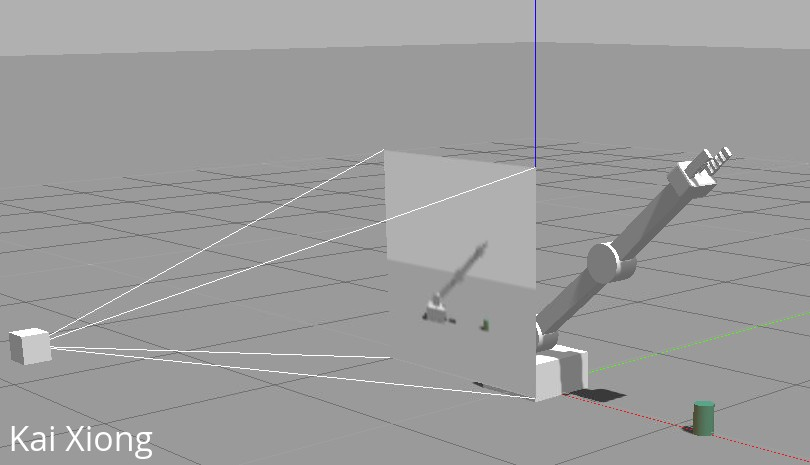
\includegraphics[scale=0.25]{robotics_arm_format.png}
      \caption{Gazebo 3-DoF robotic arm.}
      \label{fig:robot1}
\end{figure}

\section{Control Setup}
In this project, there are two options available for the robot arm kinematic control. They are positional control and velocity control. Positional control is much more simpler to use.

\begin{table}[h]
\caption{Discrete Action Encoding}
\begin{tabular}{|l|l|}
\hline
\textbf{Index} & \textbf{Action} \\ \hline
0              & J0 -            \\ \hline
1              & J0 +            \\ \hline
2              & J1 -            \\ \hline
3              & J1 +            \\ \hline
4              & J2 +            \\ \hline
5              & J2 -            \\ \hline
\end{tabular}
\end{table}

\section{Reward Function}
Deep Q-Network output is usually mapped to a particular action. The rewards system is designed to train the robot arm to touch the object of interest in one attempt. Each episode is limited to a certain number of attempts, penalty will be issued if maximum length of the episode is reached without achieving the objective. Interim reward or penalty will be issued while the robot arm is moving based on the distance from the object of interest. If the robot arm touch the object of interest, it will issue a win reward and episode is ended.

\begin{table}[h]
\begin{tabular}{|l|l|}
\hline
\textbf{Event}                    & \textbf{Rewards} \\ \hline
Ground Collision                  & -1.0             \\ \hline
Object Collision                  & -1.0             \\ \hline
End of Episode                    & -1.0             \\ \hline
Success                           & 1.0              \\ \hline
Interim Rewards                   & 5.0 x Δd         \\ \hline
Interim Distance Smoothing Factor & 0.22             \\ \hline
\end{tabular}
\caption{Rewards Function}
\label{tab:my-table}
\end{table}

\section{Hyper-parameters}
The final hyper-parameters configuration is shown in table 3. 

\begin{table}[h]
\caption{Training Hyper-parameters}
\begin{tabular}{|l|l|l|}
\hline
\textbf{Parameter} & \textbf{Value} & \textbf{Description}                                \\ \hline
Channel            & 3              & Input Image Channels (RGB)                          \\ \hline
Batch size         & 32             & Input data batch size                               \\ \hline
Replay memory      & 10000          & Size of Memory buffer for experience replay         \\ \hline
Optimizer          & Adam           & DQN Network Loss Optimizer                          \\ \hline
Learning rate      & 0.005          & Network Learning Rate                               \\ \hline
LSTM               & false          & Flag to enable Recurrent Network (LSTM)             \\ \hline
Delta              & 0.096          & Joint angle increment per step in rad (5.5 deg)     \\ \hline
EPS decay          & 400            & Epsilon delay steps                                 \\ \hline
\end{tabular}
\end{table}

\subsection{Input Dimensions}
The default input width and height parameters are 512x512. It is reduced to 128x128, as the default size was excessively large and did not provide a significant improvement. With this changes, it able to reduce the GPU memory used in training.

\subsection{Optimizer}
The Adam optimizer is widely used in vast number of different domains and the general robustness to un-tuned parameters. 

\subsection{Learning Rate}
The initial guess for the learning rate is 0.01, a lower learning rate will prevent the network to reach plateau.  

\section{Results}

\subsection{Task 1}
As for task 1, the robot arm need to the touch the object with at least a 90\% accuracy for a minimum of 100 runs. After 130 iterations, it manage to achieve more than 90\% accuracy. To watch the youtube video demonstration \href{https://youtu.be/ZcsphrfERE0}{task 1}.


\begin{figure}[thpb]
      \centering
      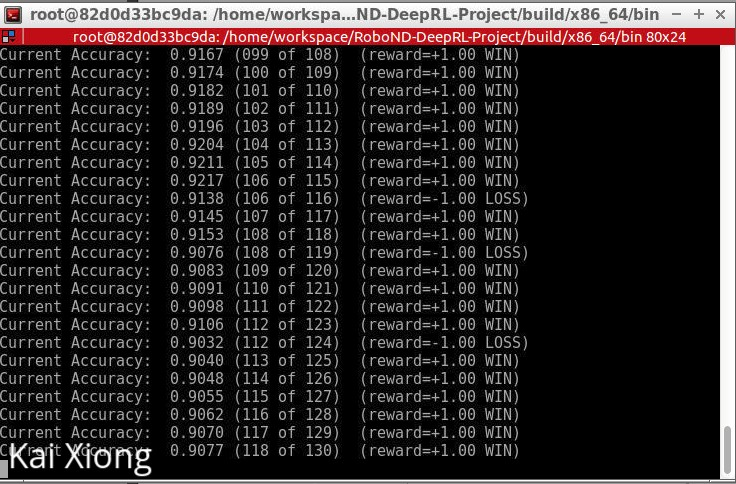
\includegraphics[scale=0.3]{task1_results_format.png}
      \caption{Snapshot log of task 1 during execution.}
      \label{fig:robot2}
\end{figure}

\subsection{Task 2}
As for task 2, the robot arm's gripper base need to touch the object with at least a 80\% accuracy for a minimum of 100 runs. After 500 iterations, it manage to achieve more than 80\%. To watch the youtube video demonstration \href{https://youtu.be/iC2EjrlD9BY}{task 2}.

\begin{figure}[thpb]
      \centering
      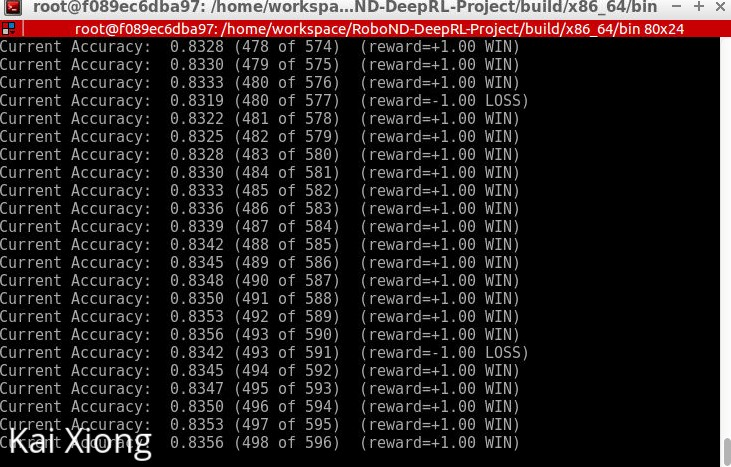
\includegraphics[scale=0.3]{task2_results_format.png}
      \caption{Snapshot log of task 2 during execution..}
      \label{fig:robot3}
\end{figure}

\section{Conclusion / Future work}
The DQN agent is capable of achieve compelling performance on two of the tasks as demonstrated above. The movement generated by the DQN network is not smooth. If the object of interest is not located in the image, the decision of the DQN network at that instant will become non-deterministic and may result in unstable oscillation. 

What methods could you use to improve on the results you got?
\begin{itemize}
      \item Implement Double Q-Learning
      \item Scaling rewards
      \item Resizing input dimensions
\end {itemize}

Would a different network configuration work better maybe? 
\begin{itemize}
      \item Yes, using a LSTM architecture. It will require a lot of training set.
\end {itemize}

Different types of control that you haven't tried yet but think could provide improvements?

\begin{itemize}
      \item Velocity control will make the robot arm movement more unstable
      \item Positional control is much simpler to use and more stable
\end {itemize}

\end{document}